\section{Calcolo Relazionale}
Il calcolo relazionale è un linguaggio di interrogazione dichiarativo: esso specifica le proprietà che devono essere soddisfatte dal risultato dell’interrogazione, senza descrivere le modalità operative per ottenerlo.

Esistono due versioni del calcolo relazionale:
\begin{itemize}
	\item il calcolo relazionale sui domini;
	\item il calcolo relazionale sulle tuple.
\end{itemize}

\paragraph{Caratteristiche del linguaggio}
Nel calcolo relazionale sulle tuple, un’interrogazione è specificata mediante una formula logica con variabili libere.  
La formula viene interpretata sul contenuto della base di dati e le variabili assumono come valori le tuple delle relazioni presenti nella base di dati.

Il calcolo relazionale sulle tuple costituisce il fondamento teorico del linguaggio SQL nella sua forma \emph{semplice}, ossia senza operatori aggregati e senza join esterni, includendo le interrogazioni nidificate.

\begin{figure}[H]
	\centering
	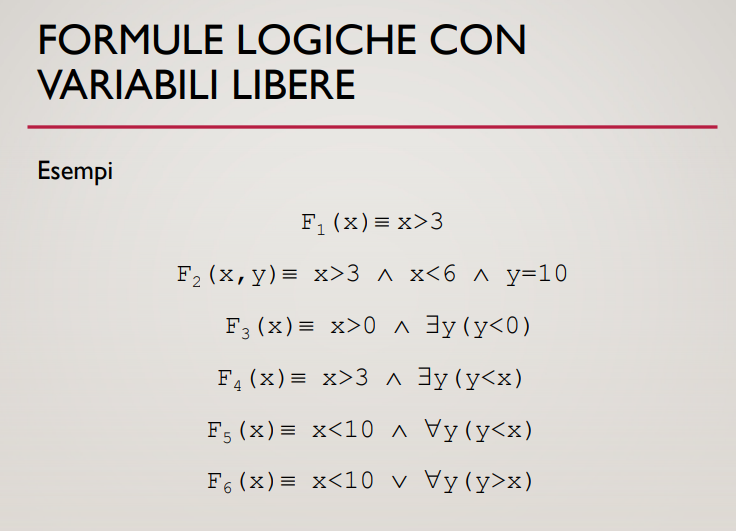
\includegraphics[width=1\linewidth]{image89}
	\caption{Esempi di formule logiche con variabili libere}
	\label{fig:image89}
\end{figure}
\paragraph{Interpretazione}
L’interpretazione consiste nella scelta degli insiemi da cui prelevare i valori da assegnare alle variabili.
Ad esempio, una formula può essere interpretata sull’insieme degli interi $\mathbb{Z}$ oppure sull’insieme dei numeri naturali $\mathbb{N}$.
\begin{figure}[H]
	\centering
	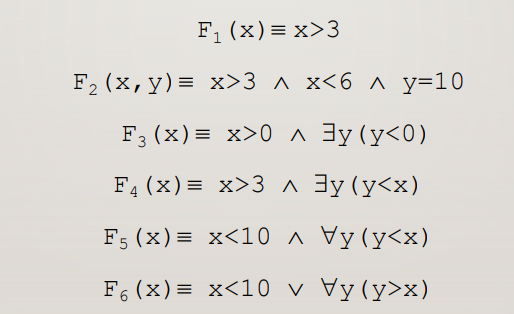
\includegraphics[width=1\linewidth]{image90}
	\caption{Formule logiche con variabili libere}
	\label{fig:image90}
\end{figure}
\paragraph{Sintassi}
Le espressioni del calcolo relazionale sulle tuple hanno la seguente forma:
\[
\{\, T \mid L \mid F \,\}
\]
dove:
\begin{itemize}
	\item \textbf{Target list} ($T$): definisce lo schema della relazione risultato e specifica come le tuple del risultato sono ottenute a partire dalle variabili libere.
	
	\item \textbf{Range list} ($L$): definisce le variabili libere e le associa alle relazioni della base di dati coinvolte nell’interrogazione.
	
	\item \textbf{Formula} ($F$): specifica la condizione logica che deve essere soddisfatta dalle variabili libere, ossia dalle tuple coinvolte nell’interrogazione.
\end{itemize}
\subsection{Sintassi}
\paragraph{Sintassi Target List}
La \textbf{target list} $T$ è una lista di elementi separati da virgole:
\[
e_1, \ldots, e_n
\]

dove ogni elemento $e_i$ può essere:
\begin{itemize}
	\item $Y : x.(Z)$,  
	dove $Y$ e $Z$ sono sequenze di attributi con la stessa cardinalità e $x$ è una variabile libera.
	
	\item $x.(Z)$,  
	dove $Z$ è una sequenza di attributi e $x$ è una variabile libera (equivalente a $Z : x.(Z)$).
	
	\item $x.*$,  
	dove $x$ è una variabile libera; in questo caso gli attributi sono tutti quelli della relazione associata alla variabile $x$ nella \emph{range list} $L$.
\end{itemize}
\paragraph{Sintassi range list}
La \textbf{range list} $L$ è una lista di elementi separati da virgole:
\[
r_1, \ldots, r_m
\]

dove ogni elemento $r_i$ ha la seguente forma:
\[
x_j(R)
\]

dove $x_j$ è una variabile libera e $R$ è il nome di una relazione dello schema della base di dati.

Per ogni variabile libera della formula $F$ esiste uno e un solo elemento $r_i$ nella \emph{range list} $L$.
\paragraph{Sintassi della formula}
La formula $F$ può essere:

\paragraph{Formula atomica}
\begin{itemize}
	\item $x.A \ \theta \ c$ \quad oppure
	\item $x_1.A_1 \ \theta \ x_2.A_2$
\end{itemize}

dove $x, x_1, x_2$ sono variabili, $A, A_1, A_2$ sono attributi, $c$ è una costante e $\theta$ è un operatore di confronto appartenente all’insieme:
\[
\{=, \neq, >, <, \geq, \leq\}.
\]

\paragraph{Formula non atomica}
\begin{itemize}
	\item se $f_1$ e $f_2$ sono formule, allora anche
	\[
	f_1 \land f_2,\quad f_1 \lor f_2,\quad \neg f_1,\quad \neg f_2
	\]
	sono formule;
	
	\item se $f$ è una formula, allora anche
	\[
	\forall x(R)\,(f) \quad \text{e} \quad \exists x(R)\,(f)
	\]
	sono formule.
\end{itemize}
\paragraph{Notazione} Variabili libere e legate nelle formule:
\begin{itemize}
	\item Nelle formule atomiche tutte le variabili sono libere.
	\item Nelle formule $\forall x\, (f)$ e $\exists x\, (f)$, la variabile $x$ è una variabile legata, mentre tutte le altre variabili mantengono lo stato (libere o legate) che avevano in $f$.
	\item Le congiunzioni, le disgiunzioni e la negazione non modificano l’insieme delle variabili libere o legate di una formula.
\end{itemize}
\subsection{Semantica}
\paragraph{Semantica}
Le formule vengono interpretate sull’istanza corrente della base di dati
\[
\mathit{db} = \{ r_1(x_1,\dots,x_n), \dots, r_m(x_1,\dots,x_n) \}.
\]
Ogni formula contiene un certo numero di variabili libere
\[
f(x_1,\dots,x_k).
\]
Data una ennupla di tuple $(t_1,\dots,t_k)$, tale ennupla rende vera la formula
quando, sostituendo le tuple $t_1,\dots,t_k$ alle variabili libere
$x_1,\dots,x_k$, la formula risulta soddisfatta.

Nel caso delle formule atomiche, una formula del tipo
\[
x_{i,A} \,\theta\, x_{j,B}
\]
è vera sulle tuple $(t_1,\dots,t_k)$ se il confronto
$t_{i,A} \,\theta\, t_{j,B}$ è soddisfatto; analogamente,
\[
x_{i,A} \,\theta\, c
\]
è vera se il confronto $t_{i,A} \,\theta\, c$ è soddisfatto, dove $\theta$ è un
operatore di confronto.

Le formule non atomiche ottenute mediante i connettivi logici
$\wedge$, $\vee$, $\neg$, $\Rightarrow$ sono vere secondo le usuali definizioni
di verità dei connettivi logici.

Per quanto riguarda i quantificatori, la formula
\[
\exists x_k\, (f)
\]
è vera sulle tuple $(t_1,\dots,t_{k-1})$ se esiste almeno una tupla $t_k$
nell’istanza di $R_k$ tale che, sostituendo $(t_1,\dots,t_k)$ alle variabili
$(x_1,\dots,x_k)$, la formula $f$ risulta vera.
Analogamente, la formula
\[
\forall x_k\, (f)
\]
è vera sulle tuple $(t_1,\dots,t_{k-1})$ se per ogni tupla $t_k$ nell’istanza di
$R_k$ la formula $f$ risulta vera quando si sostituiscono le tuple
$(t_1,\dots,t_k)$ alle variabili $(x_1,\dots,x_k)$.
\paragraph{Interpretazione di un’espressione del calcolo come interrogazione}
Un’espressione del calcolo relazionale sulle tuple può essere interpretata come
un’interrogazione della forma
\[
Q = \{\, Y_1 : x_1(Z_1), \dots, Y_k : x_k(Z_k)
\mid x_1(R_1), \dots, x_n(R_n) \mid f(x_1,\dots,x_n) \,\}.
\]

La valutazione dell’interrogazione $Q$ produce una relazione risultato $R$ tale che:
\begin{itemize}
	\item lo schema di $R$ è
	\[
	Y = Y_1 \cup \dots \cup Y_k;
	\]
	\item $R$ contiene tutte le tuple $t$ su $Y$ per le quali esiste una ennupla di
	tuple
	\[
	(t_1,\dots,t_n) \in R_1 \times \dots \times R_n
	\]
	che genera $t$ e che, sostituita alle variabili libere
	$(x_1,\dots,x_n)$, rende vera la formula $f$.
\end{itemize}
\subsection{Calcolo relazionale sulle tuple}
Il calcolo relazionale sulle tuple non è equivalente né all’algebra relazionale
né al calcolo relazionale sui domini, in quanto l’operatore di unione tra due
relazioni non è esprimibile nel calcolo relazionale sulle tuple.
Tuttavia, nel calcolo relazionale sulle tuple è possibile rappresentare sia
l’intersezione sia la differenza tra due relazioni.
\begin{figure}[H]
	\centering
	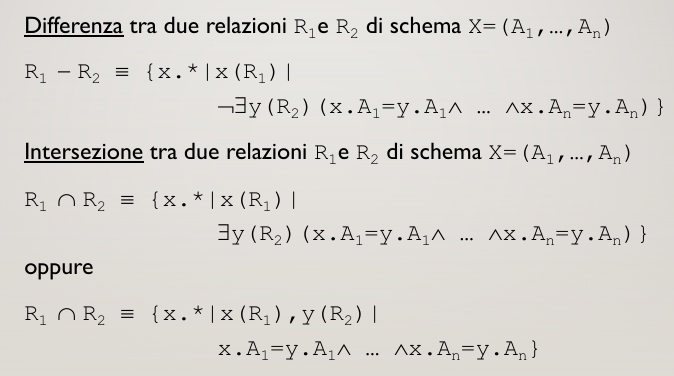
\includegraphics[width=1\linewidth]{image91}
	\caption{differenza e intersezione}
	\label{fig:image91}
\end{figure}
\begin{figure}[H]
	\centering
	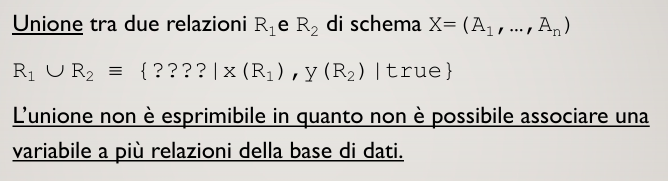
\includegraphics[width=1\linewidth]{image92}
	\caption{unione}
	\label{fig:image92}
\end{figure}
\subsection*{Esempio}
\begin{figure}[H]
	\centering
	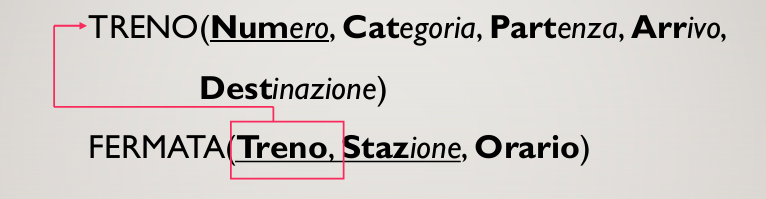
\includegraphics[width=1\linewidth]{image93}
	\caption{Progettazione Logica}
	\label{fig:image93}
\end{figure}
\begin{figure}[H]
	\centering
	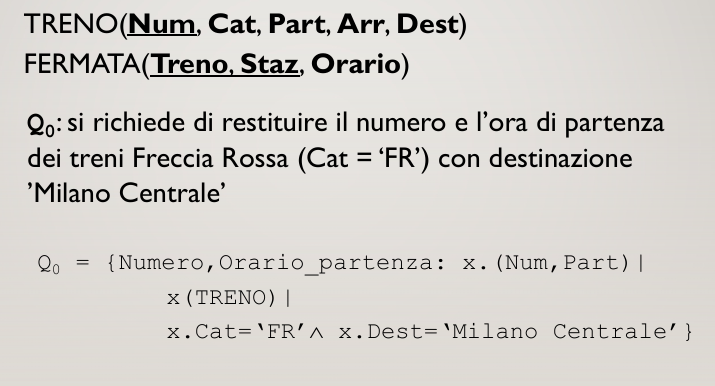
\includegraphics[width=1\linewidth]{image94}
	\caption{$Q_0$}
	\label{fig:image94}
\end{figure}
\begin{figure}[H]
	\centering
	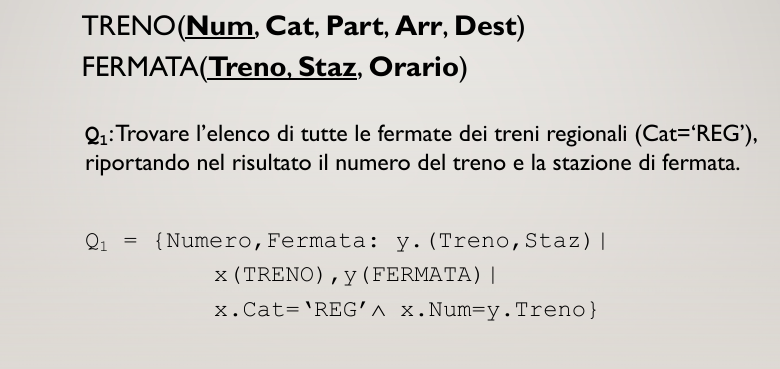
\includegraphics[width=1\linewidth]{image95}
	\caption{$Q_1$}
	\label{fig:image95}
\end{figure}

\begin{figure}[H]
	\centering
	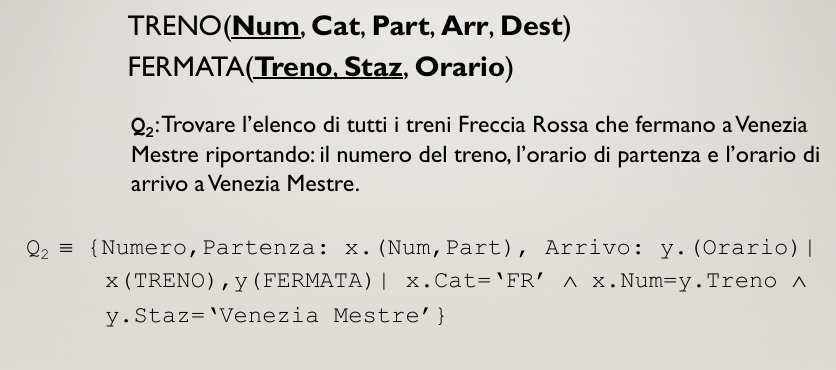
\includegraphics[width=1\linewidth]{image96}
	\caption{$Q_2$}
	\label{fig:image96}
\end{figure}
% TODO: \usepackage{graphicx} required
\begin{figure}[H]
	\centering
	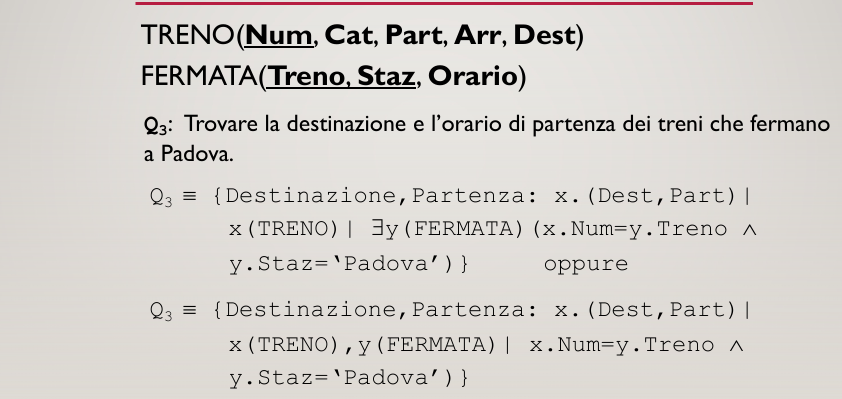
\includegraphics[width=1\linewidth]{image97}
	\caption{$Q_3$}
	\label{fig:image97}
\end{figure}
% TODO: \usepackage{graphicx} required
\begin{figure}[H]
	\centering
	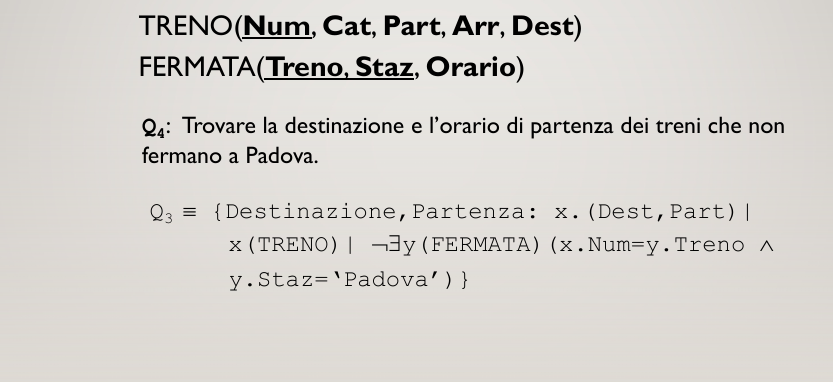
\includegraphics[width=1\linewidth]{image98}
	\caption{$Q_4$}
	\label{fig:image98}
\end{figure}
Il calcolo relazionale sulle tuple è equivalente al linguaggio di interrogazione
adottato dallo standard SQL2, se si considera la forma base delle interrogazioni
SQL, ovvero senza l’uso di operatori aggregati e di raggruppamenti.
In tale contesto, ogni espressione del calcolo relazionale sulle tuple è
direttamente traducibile in una interrogazione SQL di base.

In particolare, un’espressione del calcolo della forma
\[
\{\, T \mid L \mid F \,\}
\]
è in diretta corrispondenza con la forma base delle interrogazioni SQL:
\[
\texttt{SELECT } T \;\texttt{ FROM } L \;\texttt{ WHERE } F.
\]

La \emph{target list} $T$ individua gli attributi da restituire nel risultato
dell’interrogazione ed è mappata sulla clausola \texttt{SELECT};
la \emph{range list} $L$ specifica le relazioni coinvolte ed è mappata sulla
clausola \texttt{FROM};
infine, la formula $F$ esprime le condizioni di selezione ed è mappata sulla
clausola \texttt{WHERE}.
